\documentclass[
     11pt,         % font size
     a4paper,      % paper format
     oneside,
     ]{article}

%%%%%%%%%%%%%%%%%%%%%%%%%%%%%%%%%%%%%%%%%%%%%%%%%%%%%%%%%%%%

% PACKAGES:

% Use German :
\usepackage[USenglish]{babel}
% Input encoding
\usepackage[utf8]{inputenc}
% Font encoding
\usepackage[T1]{fontenc}
% Einbinden von URLs:
\usepackage{url}
% hyperrefs in the documents
\usepackage[bookmarks=true,colorlinks,pdfpagelabels,pdfstartview = FitH,bookmarksopen = true,bookmarksnumbered = true,linkcolor = black,plainpages = false,hypertexnames = false,citecolor = black,urlcolor=black]{hyperref} 
%\usepackage{hyperref}
% Include Graphic-files:
\usepackage{graphicx}
% Include PDF links
%\usepackage[pdftex, bookmarks=true]{hyperref}
% Fuer Textsatz
\usepackage{setspace}
% For bibliography style
\usepackage[numbers]{natbib}
% for Latex symbols
\usepackage{doc}
\usepackage[]{algorithm2e}
\usepackage{float}
\usepackage{tikz}
\usetikzlibrary{decorations.markings}
\usepackage{caption}
\usepackage{subcaption}
\usepackage{lipsum}
\usepackage{mwe}
\usepackage{pgfplots}
\usepackage{amsmath}
\usepackage{movie15}
\usepackage{hyperref}
\usepackage{mathtools}
\newcommand{\vect}[1]{\boldsymbol{#1}}

\begin{document}
	\section{Dynamic System}
	Define a 2d space $\vect{D}$,  $\vect{D}\subset \vect{R}^{2}$, $\vect{X}\in \vect{D}$.\\
	Define a 3d time-space space $\Omega$, $\Omega \subset \vect{R}^{2}\times\vect{R}$, $\vect{\xi} \in \vect{\Omega}$.
	Here $\vect{X}(t;t_{0},\vect{X}_{0}) \in \vect{D}$. $\vect{X}(t;t_{0},\vect{X}_{0})$ means if a massless particle is released at time $t_{0}$, the position of the particle at time $t$. \\
	
	$\vect{V}(\vect{X}(t;t_{0},\vect{X}_{0}),t)$ is the velocity at $\vect{X} \in D$ at time $t$ and $\vect{V}$ satisfied some level of continuity. To be specific, $\vect{V}\subset \Omega$ but with the third dimension fixed, for instance it keeps 0.04.  \\
	And dynamical system can be describe as below equations:\\
	\begin{eqnarray}
	\vect{X}^{'}(t;t_{0},\vect{X}_{0})=\vect{V}(\vect{X}(t;t_{0},\vect{X}_{0}),t)
	\end{eqnarray}
	\begin{eqnarray}
	\vect{X}(t_{0};t_{0},\vect{X}_{0})=\vect{X}_{0}
	\end{eqnarray}
	In paraview, we can show velocity by using arrow, the length of the arrow standing for the magnitude of velocity and the direction of arrow presenting the direction of velocity. By arrows, it is easy to show the velocity at any space at any time. However, it is hard to figure out how velocity changing with time. For instance, in figure\ref{fig:Overviewofvelocitydata}, getting velocity at any point is obvious, otherwise presenting velocity changing is not, i.e it is hard to show time dependency of data. 
	\begin{figure}[H]
		\centering
		\includegraphics[width=0.65\textwidth]{pic/OverviewOfVelocityData.png}
		\caption{{\tiny Overview of the Velocity Data. X, Y present the space of data, Z is time of data.}}
		\label{fig:Overviewofvelocitydata}
	\end{figure}
	\begin{figure}[H]
		\begin{minipage}{0.5\textwidth}
			\centering
			\includegraphics[width=0.5\textwidth]{pic/VelocityDataAt5s.png}
			\caption{\tiny Velocity of the space at time=5s }
			\label{fig:VelocityDataAt5s}
		\end{minipage}
		\begin{minipage}{0.5\textwidth}
			\centering
			\includegraphics[width=0.5\textwidth]{pic/VelocityDataAt7dot5s.png}
			\caption{\tiny Velocity of the space at time=7.5s}
			\label{fig:VelocityDataAt7.5s}
		\end{minipage}
	\end{figure}
	Figure\ref{fig:VelocityDataAt5s} and figure\ref{fig:VelocityDataAt7.5s} show the velocity at time 5s and time 7.5s, which describe the whole picture of velocity at those two moments and give the basic idea of how the velocity flow in the space at the exact moment. Nevertheless, at numerical situation, the translation between those two moment or during this two moments matters extremely. For instance, as to weather casting, the airflow transformation make a strongly influence on weather change. From figure\ref{fig:VelocityDataAt5s} and figure\ref{fig:VelocityDataAt7.5s}, we can only get seldom information about the transformation and there are not quantitative measurements.\\
	Recently, making a video of the data can be an alternative. The idea is getting a series of picture which present the velocity at one moment and take one picture as a frame of the video. Generally, the video reveals velocity through time dynamic and it is called velocity video. By the velocity video, people can get the rough idea of velocity changing. Taking the airflow as the example again, it is easy and fast to be aware of the center of vortex moving. Moreover, it is common and reasonable to present the vary of data, therefor making a video about velocity differential on time and the material differential about data is also a good idea.\\
	
	\section{Streamline and Pathline}

    // can insert some explain of differential on time and material differential here//\\

  
	Nowadays, streamlines and pathlines are applied into time dependency analysis of vector field visualization. \\
	Streamlines are a family of curves that are instantaneously tangent to the velocity vector of the flow. These show the direction in which a massless fluid element will travel at any point in time\cite{StreamlineDefine}. This denotes streamlines indicate  velocity at one moment. Actually, a streamline is a path traced out by a massless particle as it moves with the flow at this moment.\\
	When construct the streamline, with the flow we calculate the position of massless particle after it is released.\\
	// can insert streamline algorithm.\\
	\begin{figure}[H]
	\centering
	\includegraphics[width=0.65\textwidth]{pic/streamlineattime=5s.png}
	\caption{{\tiny some streamlines at time=5s. Arrows are the flow and those tubes are streamlines}}
	\label{fig:streamlineattime=5s}
	\end{figure}
	\begin{figure}[H]
		\centering
		\includegraphics[width=0.65\textwidth]{pic/somestreamlineattime=5s.png}
		\caption{{\tiny some streamlines at time=5s. More specific, we can see streamlines going with the flow and from those red seeds.}}
		\label{fig:somestreamlineattime=5s}
	\end{figure}
	
	Mathematically, define $\phi_{t_{0}}^{t_{n}}(\vect{X}_{0})$ as the streamline point after time $t_{n}$ start from  $\vect{X}_{0}$ at $t_{0}$. \\
	And streamline is the solution of differential equations:\\
	\begin{eqnarray}
	\frac{d\phi_{t_{0}}^{t_{n}}(\vect{X}_{0})}{dt_{n}}=V(\phi_{t_{0}}^{t_{n}}(\vect{X}_{0}),t_{0})\\
	\phi_{t_{0}}^{t_{0}}(\vect{X}_{0})=\vect{X}_{0}
	\end{eqnarray}
	As similar as streamline, pathlines are the trajectories that individual fluid particles follow. These can be thought of as "recording" the path of a fluid element in the flow over a certain period. The direction the path takes will be determined by the streamlines of the fluid at each moment in time\cite{PathlineDefine}. Basing on the definition, the difference between pathline and streamline is streamline follows the flow only at one moment, while pathline follows the  flow  through a period, i.e the velocity data field for streamline is always the velocity at time moment $t_{0}$, while the velocity data field for pathline is start from the moment $t_{0}$ and afterwards. When construct pathline, at every time step, the velocity is from different moment.\\
		\begin{figure}[H]
			\centering
			\includegraphics[width=0.65\textwidth]{pic/pathlines.png}
			\caption{{\tiny some pathlines at time=5s and end at 8s from those red seeds. we can see pathline go through the flow through time.}}
			\label{fig:pathlineatfrom5s}
		\end{figure}
	Mathematically define $\psi_{t_{0}}^{t_{n}}(X_{0})$ is the pathline point after time $t_{n}$ start from $\vect{X}_{0}$ at $t_{0}$.\\
	And pathline is the solution of differential equations:\\
	\begin{eqnarray}
		\frac{d\psi_{t_{0}}^{t_{n}}(\vect{X}_{0})}{dt}=V(\psi_{t_{0}}^{t_{n}}(\vect{X}_{0}),t_{n}+t_{0})
		\psi_{t_{0}}^{t_{0}}(\vect{X}_{0})=\vect{X}_{0}
	\end{eqnarray}
	Also, streamlines and pathlines are continuity, which means we can start streamline or pathline in any point in the streamline or pathline curve and get a completely overlapped streamline and pathline afterwards.  
	\begin{eqnarray}
	\phi_{t_{0}}^{t_{m}+t_{n}}(\vect{X}_{0})=\phi_{t_{m}+t_{0}}^{t_{n}}(\phi_{t_{0}}^{t_{m}}(\vect{X}_{0}))=\phi_{t_{n}+t_{0}}^{t_{m}}(\phi_{t_{0}}^{t_{n}}(\vect{X}_{0}))
	\end{eqnarray}
	\begin{eqnarray}
	\psi_{t_{0}}^{t_{m}+t_{n}}(\vect{X}_{0})=\psi_{t_{m}+t_{0}}^{t_{n}}(\psi_{t_{0}}^{t_{m}}(\vect{X}_{0}))=\psi_{t_{n}+t_{0}}^{t_{m}}(\psi_{t_{0}}^{t_{n}}(\vect{X}_{0}))
	\end{eqnarray}

	
	
	\section{Distance of Streamline and Pathline}

	
   \subsection{Definition}
    As we mentioned in section of streamline and pathline, the point of streamline $\phi_{t_{0}}^{t_{n}}(\vect{X}_{0})$ and the point of pathline $\psi_{t_{0}}^{t_{n}}(\vect{X}_{0})$ satisfied:
    $$	\frac{d\phi_{t_{0}}^{t_{n}}(\vect{X}_{0})}{dt_{n}}=V(\phi_{t_{0}}^{t_{n}}(\vect{X}_{0}),t_{0})$$
    	$$\phi_{t_{0}}^{t_{0}}(\vect{X}_{0})=\vect{X}_{0}$$
    $$		\frac{d\psi_{t_{0}}^{t_{n}}(\vect{X}_{0})}{dt}=V(\psi_{t_{0}}^{t_{n}}(\vect{X}_{0}),t_{n}+t_{0})$$
    $$	\psi_{t_{0}}^{t_{0}}(\vect{X}_{0})=\vect{X}_{0}$$
	Introduce a concept \textit{Distance of Streamline and Pathine after time $t_{n}$} as \textbf{$SPDis(\vect{X}_{0},t_{0},t_{n})$}. This can be used to weight time dependency characteristics of the velocity data.
	\begin{eqnarray}
	SPDis(\vect{X}_{0},t_{0},t_{n})=\biggr\lVert\phi_{t_{0}}^{t_{n}}(\vect{X}_{0})-\psi_{t_{0}}^{t_{n}}(\vect{X}_{0})\biggr\rVert
	\end{eqnarray}
	\begin{eqnarray}
	SPDis(\vect{X}_{0},t_{0},t_{n})=\int_{t=t_{0}}^{t=t_{n}+t_{0}}\biggr( V(\phi_{t_{0}}^{t}(\vect{X}_{0}),t_{0})-V(\psi_{t_{0}}^{t}(\vect{X}_{0}),t)\biggr) dt
	\end{eqnarray}
    As we can tell the $SPDis(\vect{X}_{0},t_{0},t_{n})$ depends on $V(,t_{0})$, $V(,t)$ and $t\in [t_{0},t_{0}+t_{n}]$. Therefore $SPDis(\vect{X}_{0},t_{0},t_{n})$ depends on $t$, if the position $X_{0}$, the start time $t_{0}$ and the velocity flow data are given. So at some level, \textit{Distance of Streamline and Pathine after time $t_{n}$} $SPDis(\vect{X}_{0},t_{0},t_{n})$ can measure the time dependency of the velocity flow data. There exist an simple example to show the theory.
    \begin{figure}[H]
    	\centering
    	\begin{minipage}{0.45\textwidth}
    		\centering
    		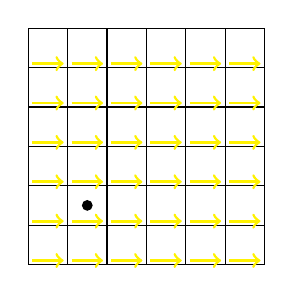
\begin{tikzpicture}[scale=0.50]
    		\foreach \x in {1,2,...,6}
    		\foreach \y in {1,...,6}
    		{
    			\draw (\x,\y) +(-.5,-.5) rectangle ++(.5,.5);
    			\draw [->,yellow,line width=1pt] (\x,\y) +(-.4,-.4) -- ++(.4,-.4);
    		}
    		\node at (2,2) [fill,circle,scale=0.2] {$A$};
    		\end{tikzpicture}
    		\caption{data at $t_{0}$ }
    		\label{$SPDis$ expalnation data at $t_{0}$}
    	\end{minipage}
    	\begin{minipage}{0.45\textwidth}
    		\centering
    		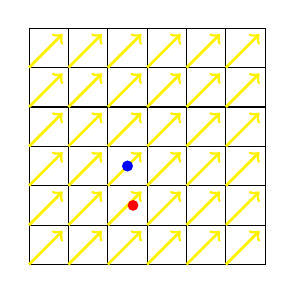
\begin{tikzpicture}[scale=0.50]
    		\foreach \x in {1,2,...,6}
    		\foreach \y in {1,...,6}
    		{
    			\draw (\x,\y) +(-.5,-.5) rectangle ++(.5,.5);
    			\draw [->,yellow,line width=1pt] (\x,\y) +(-.5,-.5) -- ++(.35,.35);
    		}
    		\node at (3.14,2) [fill,circle,red,scale=0.2] {$A$};
    		\node at (3,3) [fill,circle,blue,scale=0.2] {$B$};
    		\end{tikzpicture}
    		\caption{data at $t_{1}$ }
    		\label{$SPDis$ expalnation data at $t_{1}$}
    	\end{minipage}
    \end{figure}
    
    \begin{figure}[H]
    	\centering
    	\begin{minipage}{0.45\textwidth}
    		\centering
    		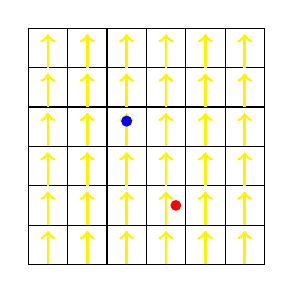
\begin{tikzpicture}[scale=0.50]
    		\foreach \x in {1,2,...,6}
    		\foreach \y in {1,...,6}
    		{
    			\draw (\x,\y) +(-.5,-.5) rectangle ++(.5,.5);
    			\draw [->,yellow,line width=1pt] (\x,\y) +(0,-.5) -- ++(0,.35);
    		}
    		\node at (4.25,2) [fill,circle,red,scale=0.2] {$A$};
    		\node at (3,4.14) [fill,circle,blue,scale=0.2] {$B$};
    		\end{tikzpicture}
    		\caption{data at $t_{2}$ }
    		\label{$SPDis$ expalnation data at $t_{2}$}
    	\end{minipage}
    	\begin{minipage}{0.45\textwidth}
    		\centering
    		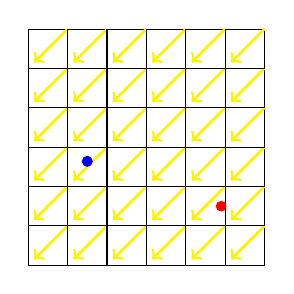
\begin{tikzpicture}[scale=0.50]
    		\foreach \x in {1,2,...,6}
    		\foreach \y in {1,...,6}
    		{
    			\draw (\x,\y) +(-.5,-.5) rectangle ++(.5,.5);
    			\draw [->,yellow,line width=1pt] (\x,\y) +(.5,.5) -- ++(-.35,-.35);
    		}
    		\node at (5.4,2) [fill,circle,red,scale=0.2] {$A$};
    		\node at (2,3.14) [fill,circle,blue,scale=0.2] {$B$};
    		\end{tikzpicture}
    		\caption{data at $t_{3}$ }
    		\label{$SPDis$ expalnation data at $t_{3}$}
    	\end{minipage}
    	\label{fig:data0&1}
    \end{figure}
    \begin{figure}[H]
    		\centering
    		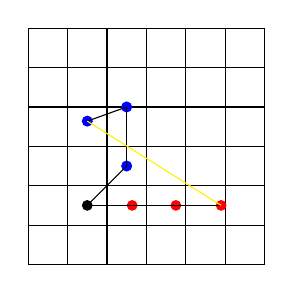
\begin{tikzpicture}[scale=0.50]
    		\foreach \x in {1,2,...,6}
    		\foreach \y in {1,...,6}
    		{
    			\draw (\x,\y) +(-.5,-.5) rectangle ++(.5,.5);
    		}
    		\node at (2,2) [fill,circle,scale=0.2] {$A$};
    		\node at (3.14,2) [fill,circle,red,scale=0.2] {$A$};
    		\node at (3,3) [fill,circle,blue,scale=0.2] {$B$};
    		\node at (4.25,2) [fill,circle,red,scale=0.2] {$A$};
    		\node at (3,4.5) [fill,circle,blue,scale=0.2] {$B$};
    		\node at (5.4,2) [fill,circle,red,scale=0.2] {$A$};
    		\node at (2,4.14) [fill,circle,blue,scale=0.2] {$B$};
    		\draw (2,2)--(3,3);
    		\draw (3,3)--(3,4.5);
    		\draw (3,4.5)-- (2,4.14);
    		\draw (2,2) .. controls (3.14,2) and (4.25,2) .. (5.4,2);
    		\draw[yellow] (5.4,2)-- (2,4.14);
    		\end{tikzpicture}
    		\caption{\tiny black line with red points is the streamline at $t_{0}$, black line with blue points is the pathline starts at $t_{0}$, black point is the seed, and the length of yellow line is the distance of end points of streamline and pathline $SPDis(X_{0},t_{3},t_{0})$}
    		\label{$SPDis$}
    \end{figure}

	Suppose, we have a simple flow data with three dimension. The data field $(S_{x},S_{y},T)$is three dimensions, two dimensions $(S_{x},S_{y})$ for 2D space and one dimension for time ($T$). The data $(V_{x},V_{y},V_{z})$ also has three dimensions, and we keeps the magnitude of velocity in 2D space $V$,i.e $\lvert V_{x},V_{y}\rvert=V=0.07$ and the magnitude in other dimension  0.04, $V_{z}=0.04$, which leads the pathline also being extended in the time dimension. Project pathline into the 2D space where streamline is and it is easy to know the $SPDis$. 
	Mathematically the flow data is defined as below:\\
	Define $V(x,y,t)$ as the velocity at point $(x,y)$ at time $t$.\\
	$V_{x}(x,y,t)$ define as velocity in $x$ direction.\\
	$V_{y}(x,y,t)$ define as velocity in $y$ direction.\\
	$V_{t}(x,y,t)$ define as velocity in $t$ direction.\\
	$V^{2}_{x}(x,y,t)+V^{2}_{y}(x,y,t)=V$, for any $(x,y,t)$.\\ 
	$V^{2}_{t}(x,y,t)=V^{'}$, for any $(x,y,t)$.\\
	$Angle(x,y,t)$ define as the angle between $(V_{x}(x,y,t),V_{y}(x,y,t))$ and $X$ direction at $t$.\\
	$Angle(x,y,t)=Angle_{0}+t*\Delta Angle$.\\
	In the example, dimension of the field is $(101,101,50)$, $V=0.07$, $V^{'}=0.04$, $Angle_{0}=30$,$\Delta Angle=2$.
	\begin{figure}[H]
		\centering
		\begin{minipage}{0.45\textwidth}
			\centering
            \includegraphics[width=0.45\textwidth]{pic/SPDisDataStart.png}
            \caption{\tiny Velocity of Example at start }
            \label{fig:VelocityofExampleAtStart}
		\end{minipage}
		\begin{minipage}{0.45\textwidth}
			\centering
			\includegraphics[width=0.45\textwidth]{pic/SPDisDataMiddle.png}
			\caption{\tiny Velocity of Example at Middle }
			\label{fig:VelocityofExampleAtMiddle}
	    \end{minipage}
		\begin{minipage}{0.45\textwidth}
			\centering
			\includegraphics[width=0.45\textwidth]{pic/SPDisDataEnd.png}
			\caption{\tiny Velocity of Example at End }
			\label{fig:VelocityofExampleAtEnd}
		\end{minipage}
	\end{figure}
	Construct pathline and streamline and, and project pathline into the 2D space where streamline is.
	\begin{figure}[H]
		\centering
		\begin{minipage}{0.65\textwidth}
		\centering
		\includegraphics[width=0.45\textwidth]{pic/streamlineandpathlineinSPdisExampleAngle2.png}
		\caption{\tiny Streamline and projected pathline when the $\Delta Angle = 2$ }
		\label{fig:StreamlineandprojectedpathlinewhentheDeltaAngle=2}
	    \end{minipage}
	    \begin{minipage}{0.65\textwidth}
	    \centering
	    \includegraphics[width=0.45\textwidth]{pic/streamlineandpathlineinSPdisExampleAngle0Dot8.png}
	    \caption{\tiny Streamline and projected pathline when the $\Delta Angle = 0.8$ }
	    \label{fig:StreamlineandprojectedpathlinewhentheDeltaAngle=0.8}
	    \end{minipage}
	\end{figure} 
	In figure\ref{fig:StreamlineandprojectedpathlinewhentheDeltaAngle=2}, use poison sampling to get some seed at beginning and construct streamline and pathline in 160 steps. It is easy to see the distance of end point of streamline and pathline which is $SPDis(\vect{Seed},t_{160})$. To compare the result, in figure\ref{fig:StreamlineandprojectedpathlinewhentheDeltaAngle=0.8}, keep every thing is the same except the $\Delta Angle=0.8$, then the $SPDis$ is smaller than it in figure\ref{fig:StreamlineandprojectedpathlinewhentheDeltaAngle=2}, because the flow in figure\ref{fig:StreamlineandprojectedpathlinewhentheDeltaAngle=2} is changing faster.
	 
\section{Normalized Distance of Streamline And Pathline}
	\subsection{Purpose} 
	 When applying $SPDisSPDis(\vect{X}_{0},t_{0},t_{n})$ to weight time dependency of data, as  we can tell the $SPDis(\vect{X}_{0},t_{0},t_{n})$ depends on $V(,t_{0})$, $V(,t)$ and $t\in [t_{0},t_{0}+t_{n}]$. so
	 the magnitude of velocity effects the result seriously, which means in some cases even the data is time dependency but $SPDis$ is smaller because of the magnitude of the data. For instance ,velocity in figure\ref*{fig:NorSPDis}, there exist two flow set, one of them is mentioned in last section with $\Delta Angle=2$ which leads the long streamline (in orange) and pathline (in blue), while the other one is the same except with $\Delta Angle=3$ and $V=0.02$. As the two flow data sets show, both of them keep the magnitude of velocity same from beginning to end with direction changing. It is obvious that data set with $\Delta Angle=3$ should be more time dependency comparing to data set with $\Delta Angle=2$. However, from  our picture, easily we can see the $SPDis$ with $\Delta Angle=3$ is smaller, which is not we desire. And what leads to this result is the other changing parameter $V$. For eliminating the effect of magnitude of $V$, introduce the concept $Normalized Streamline and pathline distance (NorSPDis)$.
	 	\begin{figure}[H]
	 		\centering
	 		\includegraphics[width=0.65\textwidth]{pic/NorSPDis.png}
	 		\caption{\tiny short pathline and streamline with $V_{0}=0.02$ and $\Delta Angle=2.5$, which is more time dependency, while the long pathline and streamline with $V_{0}=0.02$ and $\Delta Angle=2$, which is less time dependency.}
	 		\label{fig:NorSPDis}
	 	\end{figure} 
	 Definition \\
	 Therefore, define $Normalized Streamline and pathline distance (NorSPDis):$ 
	 
	 $$NorSPDis(\vect{X}_{0},t_{0},t_{n})=\frac{2*SPDis(\vect{X}_{0},t_{0},t_{n})}{Slen(n\vect{X}_{0},t_{0},t_{n})+Plen(\vect{X}_{0},t_{0},t_{n})}$$
	 
	As we know from last section $$	SPDis(\vect{X}_{0},t_{0},t_{n})=\int_{t=t_{0}}^{t=t_{n}+t_{0}}\biggr\lVert V(\phi_{t_{0}}^{t}(\vect{X}_{0}),t_{0})-V(\psi_{t_{0}}^{t}(\vect{X}_{0}),t)\biggr\rVert dt$$
	Convert to discrete construction algorithm:\\
	 $$	SPDis(\vect{X}_{0},t_{0},t_{n})=\sum_{i=0}^{i=n}\biggr\lVert V(\phi_{t_{0}}^{t_{i}}(\vect{X}_{0}),t_{0})-V(\psi_{t_{0}}^{t_{i}}(\vect{X}_{0}),t_{i})\biggr\rVert\times\Delta t_{i}$$
	 
	 $Slen(\vect{X}_{0},t_{0},t_{n})$: The length of streamline at $t_{n}$ which started at $\vect{X}_{0},t_{0}$ at $t_{n}$.
	 $$Slen(\vect{X}_{0},t_{0},t_{n})=\sum_{i=1}^{i=n}\biggr\lVert\phi_{t_{0}}^{t_{i}}(X_{0})-\phi_{t_{0}}^{t_{i-1}}(X_{0})\biggr\rVert$$
	 where:\\
	 $$\phi_{t_{0}}^{t_{i}}(X_{0})=V(\phi_{t_{0}}^{t_{i-1}}(X_{0}),t_{0})\times\Delta t_{i}+\phi_{t_{0}}^{t_{i-1}}(X_{0})$$
	 $$Slen(\vect{X}_{0},t_{0},t_{n})=\sum_{i=1}^{i=n}(V(\phi_{t_{0}}^{t_{i-1}}(X_{0}),t_{0})\times\Delta t_{i})$$
	 As similar:\\
	 $Plen(\vect{X}_{0},t_{0},t_{n})$: The length of pathline at $t_{n}$ which started at $\vect{X}_{0},t_{0}$ at $t_{n}$.
	 $$Plen(\vect{X}_{0},t_{0},t_{n})=\sum_{i=1}^{i=n}\biggr\lVert\psi_{t_{0}}^{t_{i}}(X_{0})-\psi_{t_{0}}^{t_{i-1}}(X_{0})\biggr\rVert$$
	 $$\psi_{t_{0}}^{t_{i}}(X_{0})=V(\psi_{t_{0}}^{t_{i-1}}(X_{0}),t_{i-1})\times\Delta t_{i}+\psi_{t_{0}}^{t_{i-1}}(X_{0})$$
	 $$Plen(\vect{X}_{0},t_{0},t_{n})=\sum_{i=1}^{i=n}(V(\psi_{t_{0}}^{t_{i-1}}(X_{0}),t_{i-1})\times\Delta t)$$
	 where $t_{i}<=t_{n}$, and $\Delta_{i} t=t_{i}-t_{i-1}$ is the time step at $t_{i-1}$.
	 
	 
	 $$NorSPDis(\vect{X}_{0},t_{0},t_{n})=\frac{2SPDis(\vect{X}_{0},t_{0},t_{n})}{Slen(n\vect{X}_{0},t_{0},t_{n})+Plen(\vect{X}_{0},t_{0},t_{n})}$$
	 $$=2\frac{\sum_{i=0}^{i=n}\biggr\lVert V(\phi_{t_{0}}^{t_{i}}(\vect{X}_{0}),t_{0})-V(\psi_{t_{0}}^{t_{i}}(\vect{X}_{0}),t_{i})\biggr\rVert\times\Delta t_{i}}{\sum_{i=1}^{i=n}(V(\phi_{t_{0}}^{t_{i-1}}(X_{0}),t_{0})\times\Delta t_{i})+\sum_{i=1}^{i=n}(V(\psi_{t_{0}}^{t_{i-1}}(X_{0}),t_{i-1})\times\Delta t_{i})}$$
	 $$=2\frac{\sum_{i=0}^{i=n}\biggr\lVert V(\phi_{t_{0}}^{t_{i}}(\vect{X}_{0}),t_{0})-V(\psi_{t_{0}}^{t_{i}}(\vect{X}_{0}),t_{i})\biggr\rVert\times\Delta t_{i}}{\sum_{i=1}^{i=n}(V(\phi_{t_{0}}^{t_{i-1}}(X_{0}),t_{0}))+(V(\psi_{t_{0}}^{t_{i-1}}(X_{0}),t_{i-1}))\times\Delta t_{i}}$$
	 Dived by $V(\vect{X}_{0},t_{0})$
	 we get:\\
	 $$=2\frac{\sum_{i=0}^{i=n}\biggr\lVert V_{\Delta}(\phi_{t_{0}}^{t_{i}}(\vect{X}_{0}),t_{0})-V_{\Delta}(\psi_{t_{0}}^{t_{i}}(\vect{X}_{0}),t_{i})\biggr\rVert\times\Delta t_{i}}{\sum_{i=1}^{i=n}(V_{\Delta}(\phi_{t_{0}}^{t_{i-1}}(X_{0}),t_{0}))+(V_{\Delta}(\psi_{t_{0}}^{t_{i-1}}(X_{0}),t_{i-1}))\times\Delta t_{i}}$$
	 And $V_{\Delta}=\frac{V(.)}{V(\vect{X}_{0},t_{0})}$, which only represent changing of velocity. so
	 At some level we can eliminate the $V$ effect.
	 //insert the result of Normal Distance figure

\section{Sum And Average Distance of Streamline And Pathline}

	In some area, this case usually happens,i.e the value of $SPDis(\vect{X}_{0},t_{0},t_{n})$ is random in some level. For example, even $SPDis(\vect{X}_{0},t_{0},t_{n})$ is small, but it is possible that during time step $t_{0}$ to $t_{n}$, after some time  $_{m}$, $SPDis(\vect{X}_{0},t_{0},t_{m})$ is great which means data is very time dependency. For eliminating the random characteristics if $SPDis(\vect{X}_{0},t_{0},t_{n})$, we measure $Sum Distance of Streamline And Pathine (SumSPDis(\vect{X}_{0},t_{0},t_{n}))$ or  $Sum Normalized Distance of Streamline And Pathine (SumNorSPDis(\vect{X}_{0},t_{0},t_{n}))$.

	Generate a simple vortex data set, which keeps the core of vortex at the same point and the magnitude of $V$ keep increasing in the same $Delta V$.\\ 
	\begin{figure}[H]
		\centering
		\includegraphics[width=0.75\textwidth]{pic/SumData.png}
		\caption{{\tiny vortex data.}}
		\label{fig:SumVortexData}
	\end{figure}
		\begin{figure}[H]
			\centering
			\begin{minipage}{0.45\textwidth}
				\centering
				\includegraphics[width=0.45\textwidth]{pic/SumSPDist=1s.png}
				\caption{\tiny a streamline and a pathline start at(25,50,10) go through 1s }
				\label{fig:SumSPDist=1s}
			\end{minipage}
				\begin{minipage}{0.45\textwidth}
					\centering
					\includegraphics[width=0.45\textwidth]{pic/SumSPDist=2s.png}
					\caption{\tiny a streamline and a pathline start at(25,50,10) go through 2s }
					\label{fig:SumSPDist=2s}
				\end{minipage}
		\end{figure}

	Exactly because the case in figure\ref{fig:SumSPDist=1s} and figure\ref{fig:SumSPDist=2s}, the $SPDis$ can be more casual because of the start seed and time. For example the $SPDis$ in figure\ref{fig:SumSPDist=1s} is much greater than in figure\ref{fig:SumSPDist=2s}, which is nonsense because the velocity in both of them have the same time dependency. So we define $SumSPDis$ and $AveSPDis$ to eliminate the randomly part of the $SPDis$. As the same reason as we mentioned in last section, we also define $SumNorSPDis$ and $AveNorSPDis$.\\
	\begin{itemize}
		\item $SumSPDis$
		$$SumSPDis(\vect{X}_{0},t_{0},t_{n})=\int_{t=t_{0}}^{t=t_{n}+t_{0}} SPDis(\vect{X}_{0},t_{0},t)dt$$
		\item $AveSPDis$
			$$AveSPDis(\vect{X}_{0},t_{0},t_{n})=\frac{1}{t_{n}}\int_{t=t_{0}}^{t=t_{n}+t_{0}} SPDis(\vect{X}_{0},t_{0},t)dt$$
		\item $SumNorSPDis$
		$$SumNorSPDis(\vect{X}_{0},t_{0},t_{n})=\int_{t=t_{0}}^{t=t_{n}+t_{0}} NorSPDis(\vect{X}_{0},t_{0},t)dt$$
		\item $AveNorSPDis$
				$$AveNorSPDis(\vect{X}_{0},t_{0},t_{n})=\frac{1}{t_{n}}\int_{t=t_{0}}^{t=t_{n}+t_{0}} NorSPDis(\vect{X}_{0},t_{0},t)dt$$
	\end{itemize}
	
	    \begin{figure}[H]
	    	\centering
	    	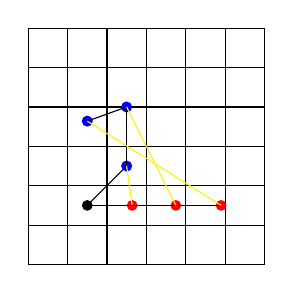
\begin{tikzpicture}[scale=0.50]
	    	\foreach \x in {1,2,...,6}
	    	\foreach \y in {1,...,6}
	    	{
	    		\draw (\x,\y) +(-.5,-.5) rectangle ++(.5,.5);
	    	}
	    	\node at (2,2) [fill,circle,scale=0.2] {$A$};
	    	\node at (3.14,2) [fill,circle,red,scale=0.2] {$A$};
	    	\node at (3,3) [fill,circle,blue,scale=0.2] {$B$};
	    	\node at (4.25,2) [fill,circle,red,scale=0.2] {$A$};
	    	\node at (3,4.5) [fill,circle,blue,scale=0.2] {$B$};
	    	\node at (5.4,2) [fill,circle,red,scale=0.2] {$A$};
	    	\node at (2,4.14) [fill,circle,blue,scale=0.2] {$B$};
	    	\draw (2,2)--(3,3);
	    	\draw (3,3)--(3,4.5);
	    	\draw (3,4.5)-- (2,4.14);
	    	\draw (2,2) .. controls (3.14,2) and (4.25,2) .. (5.4,2);
	    	\draw[yellow] (5.4,2)-- (2,4.14);
	    	\draw[yellow] (3,3)-- (3.14,2);
	    	\draw[yellow] (3,4.5)-- (4.25,2);
	    	\end{tikzpicture}
	    	\caption{\tiny black line with red points is the streamline at $t_{0}$, black line with blue points is the pathline starts at $t_{0}$, black point is the seed, and the lengths of yellow lines are the distance of end points of streamline and pathline $SPDis(X_{0},t_{1},t_{0})$,$SPDis(X_{0},t_{2},t_{0})$,$SPDis(X_{0},t_{3},t_{0})$, sum up those three length is the $SumSPDis$}
	    	\label{$SumSPDis$}
	    \end{figure}
	Apply $SumSPDis$ on the data set described before. Get the result as picture below shown:
			\begin{figure}[H]
				\centering
				\begin{minipage}{0.45\textwidth}
					\centering
					\includegraphics[width=0.45\textwidth]{pic/sumdisforsumdata.png}
					\caption{\tiny $SumSPDis$ of seeds at the time 0.25s and streamline and pathline go through 2.25s}
					\label{fig:sumdisforsumdata}
				\end{minipage}
				\begin{minipage}{0.45\textwidth}
					\centering
					\includegraphics[width=0.45\textwidth]{pic/disforsumdata.png}
					\caption{\tiny $SPDis$ of seeds at the time 0.25s and streamline and pathline go through 2.25s}
					\label{fig:disforsumdata}
				\end{minipage}
			\end{figure}
	Basing on the data information, time dependency of seeds with the same distance to the center. In figure\ref{fig:sumdisforsumdata}, we can see the case, while in figure\ref{fig:disforsumdata} this is not shown, as in some area the case in figure\ref{fig:SumSPDist=2s} happens.
	

\section{Exponent Regression of Distances of Streamlines And Pathlines}

   Purpose\\
	When construct the streamline and pathline, $SPDis(\vect{X}_{0},t_{0},t_{i})$ maybe changes a lot with time. So it is a little rush to say the data along the streamline and pathline is time dependent base on a  $SPDis(\vect{X}_{0},t_{0},t_{n})$. For example, there can be a case, $SPDis(\vect{X}_{0},t_{0},t_{i})$ , when $t_{i}\in[t_{0},t_{0}+\frac{t_{n}}{2}]$ is great, but at another half time the $SPDis(\vect{X}_{0},t_{0},t_{i})$  become smaller, if we only use $SPDis(\vect{X}_{0},t_{0},t_{n})$ to weight time dependency, then possibly it is not accurate.
	\begin{figure}[H]
	 		\centering
	 		\includegraphics[width=0.75\textwidth]{pic/SPdisPlot.png}
	 		\caption{{\tiny SPDis Plot at X=49 Y=28 Time from250 go 2s.}}
	 		\label{fig:SPdisPlot}
	\end{figure}
	In the figure\ref{fig:SPdisPlot}, we can not say it is not time dependency just because  $SPDis(\vect{X}_{0},t_{0},t_{n})$ is small. We can show the streamline and pathline from this seed. From the figure, it is easy to say it is time dependent.
		\begin{figure}[H]
			\centering
			\begin{minipage}{0.45\textwidth}
							\centering
							\includegraphics[width=0.65\textwidth]{pic/streamlineandpathlinex=49y=28from250go2sExponetcase.png}
							\caption{{\tiny streamline and pathline at X=49 Y=28 Time from250 go 2s.}}
							\label{fig:streamlineandpathlinex=49y=28from250go2sExponetcase}
			\end{minipage}
						\begin{minipage}{0.45\textwidth}
							\centering
							\includegraphics[width=0.65\textwidth]{pic/streamlineandpathlinex=49y=20from250go2sExponetcase.png}
							\caption{{\tiny streamline and pathline at X=49 Y=20 Time from250 go 2s.}}
							\label{fig:streamlineandpathlinex=49y=20from250go2sExponetcase}
						\end{minipage}

		\end{figure}
	So we introduce Exponent Regression of Distances of Streamlines And Pathlines to explain the generate time dependency of the data during the time.
	 Definition\\
	First get the data sample for regression. Divide the time range $[t_{0},t_{0}+t_{n}]$ uniformly, get time  $t_{1}$, $t_{2}$, ..., $t_{i}$,..., $t_{n}$ after $t_{0}$ and computing $SPDis(\vect{X}_{0},t_{0},t_{i})$ for them, called $SPDis_{i}$.\\
	Define regression mode:
	$$f(t_{i})=\lambda e^{t_{i}}-\lambda$$ $i\in [1,n]$
	Using least square to get $\lambda$, set the goal function $F(\lambda)$:
	$$F(\lambda)=\sum_{i=1}^{i=n}(\lambda e^{t_{i}}-\lambda-SPDis_{i})^{2}$$
	And then $$\min_{\lambda} F(\lambda)$$
	Differential on $\lambda$
	$$F^{'}(\lambda)=\sum_{i=1}^{i=n}2(\lambda e^{t_{i}}-\lambda-SPDis_{i})(e^{\lambda}-1)$$
	Let $F^{'}(\lambda)=0$
	And get the $/lambda$:
	\begin{eqnarray}
	\lambda=\frac{\sum_{i=1}^{i=n}SPDis_{i}(e^{t_{i}}-1)}{\sum_{i=1}^{i=n}(e^{t_{i}}-1)}
	\end{eqnarray}
	Call the $\lambda$ \textbf{Increasing Exponent of Time Dependency}.
Result\\
	Compare two plots of $SPDis$, the green one is the example before, and blue one is another $SPDis$ of the seed beside the seed of the blue one.
			\begin{figure}[H]
				\centering
				\includegraphics[width=0.65\textwidth]{pic/spdisplotcomparebluex=49y=20greeny=28.png}
				\caption{{\tiny SPDis Plot at X=49 Y=28(green) and Y=20(blue) Time from250 go 2s. }}
				\label{fig:spdisplotcomparebluex=49y=20greeny=28}
			\end{figure}
			
			
	           \begin{figure}[H]
						\centering
						\begin{minipage}{0.65\textwidth}
							\centering
							\includegraphics[width=0.65\textwidth]{pic/SPDisStart250Go80.png}
							\caption{{\tiny SPDisStart250Go80 Green one $\lambda=0.00754665$, blue one $\lambda=0.0117781$}}
							\label{fig:SPDisStart250Go80}
						\end{minipage}
						\begin{minipage}{0.65\textwidth}
							\centering
							\includegraphics[width=0.65\textwidth]{pic/LamdaStart250Go80.png}
							\caption{{\tiny Lamda Start250 Go80}}
							\label{fig:LamdaStart250Go80}
						\end{minipage}
						
					\end{figure}
					
		We extract the main obvious difference part, can check how are streamlines and pathlines. 
				
					
					
					\begin{figure}[H]
						\centering
						\begin{minipage}{0.45\textwidth}
							\centering
							\includegraphics[width=0.65\textwidth]{pic/streamlinepathlinex=30-40y=37Start250Go80.png}
							\caption{\tiny streamlinepathlinex=30-40y=37Start250Go80 }
							\label{fig:streamlinepathlinex=30-40y=37Start250Go80}
						\end{minipage}
						\begin{minipage}{0.45\textwidth}
							\centering
							\includegraphics[width=0.65\textwidth]{pic/SPDisPlotX=30,40Y=37Start250Go80.png}
							\caption{\tiny SPDisPlotX=30,40Y=37Start250Go80, Green one $\lambda=0.0171302$, blue one $\lambda=0.00887767$}
							\label{fig:SPDisPlotX=30,40Y=37Start250Go80}
						\end{minipage}
						
					\end{figure}
	
	


\section{Sum Distance Difference of Streamline and Pathline}
As we mentioned before:
\begin{eqnarray}
	SPDis(\vect{X}_{0},t_{0},t_{n})=\int_{t=t_{0}}^{t=t_{n}+t_{0}}\biggr( V(\phi_{t_{0}}^{t}(\vect{X}_{0}),t_{0})-V(\psi_{t_{0}}^{t}(\vect{X}_{0}),t)\biggr) dt
\end{eqnarray}
However, there is a problem that when the $SPDis((\vect{X}_{0},t_{0},t_{i}))$ decrease, it is hard to say data is less time dependency. Then define a parameter called $Distance Difference(\vect{X}_{0},t_{0},t_{i})$:
\begin{eqnarray}
DisDiff(\vect{X}_{0},t_{0},t_{i})=\biggr\lvert SPDis(\vect{X}_{0},t_{0},t_{i})-SPDis(\vect{X}_{0},t_{0},t_{i-1})\biggr\rvert\\
=\int_{t=t_{i-1}+t_{0}}^{t=t_{i}+t_{0}}\biggr\lvert V(\phi_{t_{0}}^{t}(\vect{X}_{0}),t_{0})-V(\psi_{t_{0}}^{t}(\vect{X}_{0}),t)\biggr\rvert dt
\end{eqnarray}
This measure how does the velocity data along the streamline and pathline change at every moment. Then we define Sum Distance Difference of Streamline and Pathline from $t_{0}$ to $t_{0}+t_{n}$ as below:
 \begin{eqnarray}
 SumDisDiff(\vect{X}_{0},t_{0},t_{i})=\biggr\lvert SPDis(\vect{X}_{0},t_{0},t_{i})-SPDis(\vect{X}_{0},t_{0},t_{i-1})\biggr\rvert\\
 =\int_{t=t_{i-1}+t_{0}}^{t=t_{i}+t_{0}}\biggr\lvert V(\phi_{t_{0}}^{t}(\vect{X}_{0}),t_{0})-V(\psi_{t_{0}}^{t}(\vect{X}_{0}),t)\biggr\rvert dt
 \end{eqnarray}
 
\begin{figure}[H]
	\centering
 	\begin{minipage}{0.65\textwidth}
 		\centering
 		\includegraphics[width=0.65\textwidth]{pic/SumDisDiffstart250go80.png}
 		\caption{\tiny Sum Distance Difference start at time 250 and go 2s. The area in read cycle is most different area compare to $SPDis$. The area in green cycle shows the specific structure of the data }
 		\label{fig:SumDisDiffstart250go80}
 	\end{minipage}
 	\begin{minipage}{0.65\textwidth}
 		\centering
 		\includegraphics[width=0.65\textwidth]{pic/sumdisdiffstreamlinepathlinex=75-90y=65-72start250go2s.png}
 		\caption{\tiny Streamline and pathline at x=75-90y=65-72start250 go 2s to show it is very time dependency at this area}
 		\label{fig:sumdisdiffstreamlinepathlinex=75-90y=65-72start250go2s}
 		\end{minipage}						
\end{figure}
As the equation shows, it integral all the change at every step in absolute, so in this algorithm it shows all those parts with high time dependency characteristic. From the figure\ref{fig:SumDisDiffstart250go80}, it is easy to tell there are more parts in red. Moreover, it has clearer and more specific structure, for example the green cycle part in the figure\label{fig:SumDisDiffstart250go80}.
\begin{figure}[H]
	\centering
	\begin{minipage}{0.65\textwidth}
		\centering
		\includegraphics[width=0.65\textwidth]{pic/sumdisdiffstreamlinepathlinex=779-80y=6-7start250go2s.png}
		\caption{\tiny Sum Distance Difference start at time 250 and go 2s. The area in read cycle is most different area compare to $SPDis$. The area in green cycle shows the specific structure of the data }
		\label{fig:sumdisdiffstreamlinepathlinex=779-80y=6-7start250go2s}
	\end{minipage}
	\begin{minipage}{0.65\textwidth}
		\centering
		\includegraphics[width=0.65\textwidth]{pic/sumdisdiffstreamlinepathlinex=779-80y=14-15start250go2s.png}
		\caption{\tiny Streamline and pathline at x=75-90y=65-72start250 go 2s to show it is very time dependency at this area}
		\label{fig:sumdisdiffstreamlinepathlinex=779-80y=14-15start250go2s}
	\end{minipage}						
\end{figure}
Comparing this two kinds of streamline and pathline, in figure\ref{fig:sumdisdiffstreamlinepathlinex=779-80y=6-7start250go2s}, the $SumDisDiff$ of seeds is not as big as seed in figure\ref{fig:sumdisdiffstreamlinepathlinex=779-80y=14-15start250go2s}. However, we can tell that the $SPDis$ is almost the same,but as the velocity data along the curve changing more at most step, because the pathline is much longer in \ref{fig:sumdisdiffstreamlinepathlinex=779-80y=14-15start250go2s}.









\section{Analyze Time Dependency of the Whole Data}

 Purpose\\
	For detecting the time dependency characteristics of the whole data, and get the general idea of the whole data about time dependency characteristics. We introduce some parameters here.
 Definition \\
	\begin{itemize}
		\item Maximum (Minimum) Distance of Streamline And Pathline $MaxSPDis(\vect{X}_{0},t_{0},t_{n})$ and $MinSPDis(\vect{X}_{0},t_{0},t_{n})$:\\
		Computing the $SPDis(\vect{X}_{0},t_{0},t)$ from $ t_{0} $ to $t_{n}$ when construct the streamline and pathine, and pick the maximum and minimum.
		$$MaxSPDis(\vect{X}_{0},t_{0},t_{n})=\max_{t} SPDis(\vect{X}_{0},t_{0},t)$$
		$$MinSPDis(\vect{X}_{0},t_{0},t_{n})=\min_{t} SPDis(\vect{X}_{0},t_{0},t)$$
		\item Maximum (Minimum) Normalized Distance of Streamline And Pathline $MaxNorSPDis(\vect{X}_{0},t_{0},t_{n})$ and $MinNorSPDis(\vect{X}_{0},t_{0},t_{n})$:\\
		Computing the $NorSPDis(\vect{X}_{0},t_{0},t)$ at every time from $t_{0}$ to $t_{n}$ when construct the streamline and pathine, and pick the maximum and minimum.
		$$MaxNorSPDis(\vect{X}_{0},t_{0},t_{n})=\max_{t} NorSPDis(\vect{X}_{0},t_{0},t)$$
		$$MinNorSPDis(\vect{X}_{0},t_{0},t_{n})=\min_{t} NorSPDis(\vect{X}_{0},t_{0},t)$$
		\item Percentage of $SPDis(\vect{X}_{0},t_{0},t_{n})$ Smaller than Threshold $PerSPDis(\vect{X}_{0},t_{0},t_{n})$\\
		Set a parameter which is called \textit{distance threshold} $\mu$. Count the percentage of time when the $SPDis(\vect{X}_{0},t_{0},t)$  is less than the parameter.
		$$ PerSPDis(\vect{X}_{0},t_{0},t_{n})=\frac{\int_{t=t_{0}}^{t=t_{n}}(\mu-SPDis(\vect{X}_{0},t_{0},t)>0)}{t_{n}-t_{0}}$$
	\end{itemize} 
 Result Analysis\\
	\begin{tabular}{ l | l | l | l | l| l }
		Time Dependency& MaxSPdis & MinSPDis & MaxNorSPDis & MinNorSPDis & PerSPDid \\
		More & Great & Undefined & Great & Undefined & Small \\
		Less & Small & Small & Small& Small & Great\\
	\end{tabular}
\section{Distance of Streamlines Comparison}

 Purpose\\
	Computing $SPDis(\vect{X}_{0},t_{0},t_{n})$ or $NorSPDis(\vect{X}_{0},t_{0},t_{n})$ compares the streamline and pathline which shows time dependency characteristics of data during the time $[t_{0},t_{n}]$. However, in some case, for example during the time $[t_{0},t_{n}]$, the data in the start area ($X_{0}$ area) swings a lot i.e change to other state and change back, if the result we want to know is about the data change between two specific time. Then $SPDis(\vect{X}_{0},t_{0},t_{n})$ leads a big mistake, because perhaps as the data changed during the time, pathline goes to far away as pathine is a curve integrated.For example from one vortex to another vortex, then the pathline will go away from the area, but the streamline even at the end time will still at this area with a little change.\\ So here define streamline comparison.
	
	\begin{figure}[H]
			\centering
			\includegraphics[width=0.65\textwidth]{pic/streamlinecompareexample.png}
			\caption{streamlines at two moments are similar, but pathline go through those  two moments change a lot }
			\label{fig:streamlinecompareexample}
		\end{figure}
	\begin{figure}[H]
		\centering
		
		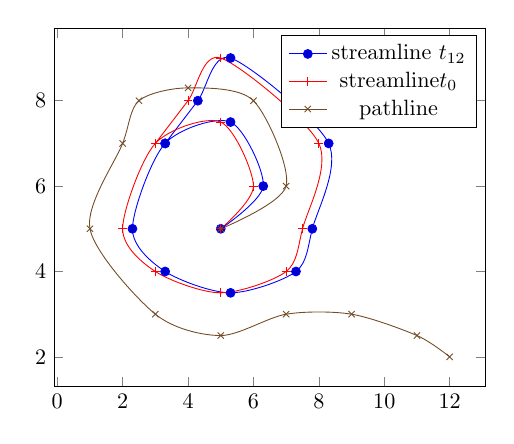
\begin{tikzpicture}[scale=0.8]
		
		\begin{axis}
		\addplot+[smooth,mark=*] plot coordinates
		{ (5,5) (6.3,6) (5.3,7.5) (3.3,7) (2.3,5) (3.3,4) (5.3,3.5) (7.3,4) (7.8,5) (8.3,7) (5.3,9) (4.3,8) (3.3,7) };
		\addlegendentry{streamline $t_{12}$ }
		
		\addplot+[smooth,mark=+] plot coordinates
		{ (5,5) (6,6) (5,7.5) (3,7) (2,5) (3,4) (5,3.5) (7,4) (7.5,5) (8,7) (5,9) (4,8) (3,7) };
		\addlegendentry{streamline$t_{0}$ }
		\addplot+[smooth,mark=x] plot coordinates
		{ (5,5) (7,6) (6,8) (4,8.3) (2.5,8) (2,7) (1,5) (3,3) (5,2.5) (7,3) (9,3) (11,2.5) (12,2)};
		\addlegendentry{pathline}
		\end{axis}
		\end{tikzpicture}
		
		\caption{Streamlines changed a little but pathine changed a lot}
		\label{when we use streamline to streamline}
	\end{figure}
 Definition\\
	$\phi_{t_{0}}^{t_{i}}(X_{0},T_{1})$ is the the point of the streamline at time $t_{i}$ start from $X_{0}$ at $T_{1}$.\\
	$\phi_{t_{0}}^{t_{i}}(X_{0},T_{2})$ is the the point in the streamline at time $t_{i}$ start from $X_{0}$ at $T_{2}$.\\
	Still we have in the dynamic system:\\
	\begin{eqnarray}
	\phi_{t_{0}}^{t_{m}+t_{n}}(\vect{X}_{0},T_{1})=\phi_{t_{m}+t_{0}}^{t_{n}}(\phi_{t_{0}}^{t_{m}}(\vect{X}_{0},T_{1}))=\phi_{t_{n}+t_{0}}^{t_{m}}(\phi_{t_{0}}^{t_{n}}(\vect{X}_{0},T_{1}))\\
	\phi_{t_{0}}^{t_{0}}(X_{0},T_{1})=X_{0}\\
	\phi_{t_{0}}^{t_{m}+t_{n}}(\vect{X}_{0},T_{2})=\phi_{t_{m}+t_{0}}^{t_{n}}(\phi_{t_{0}}^{t_{m}}(\vect{X}_{0},T_{2}))=\phi_{t_{n}+t_{0}}^{t_{m}}(\phi_{t_{0}}^{t_{n}}(\vect{X}_{0},T_{2}))\\
	\phi_{t_{0}}^{t_{0}}(X_{0},T_{2})=X_{0}\\
	\end{eqnarray}
	And define $Distance of Streamline (SSDis(\vect{X}_{0},t_{n},T_{1},T_{2}))$ as distance of points at time $t_{n}$ streamlines start at $X_{0}$ at $ T_{1} $ and $ T_{2} $.
	$$SSDis(\vect{X}_{0},t_{n},T_{1},T_{2})=\biggr\lVert \phi_{t_{0}}^{t_{i}}(X_{0},T_{1})-\phi_{t_{0}}^{t_{i}}(X_{0},T_{2})\biggr\rVert$$
	As similar as $NorSSdis(\vect{X}_{0},t_{n},T_{1},T_{2})$, define:
	$$NorSSDis(\vect{X}_{0},t_{n},T_{1},T_{2})=2*\frac{SSDis(\vect{X}_{0},t_{n},T_{1},T_{2})}{Slen(\vect{X}_{0},t_{n},T_{1})+Slen(\vect{X}_{0},t_{n},T_{2})}$$
	where $Sle1$ is length of streamline start $T$ along the curve.
	$$Slen(\vect{X}_{0},t_{n},T_{1},T)=\sum_{i=1}^{i=n}\biggr\lVert\phi_{t_{0}}^{t_{i}}(X_{0},T)-\phi_{t_{0}}^{t_{i-1}}(X_{0},T)\biggr\rVert$$
	where $t_{i}<=t_{n}$, and $t_{i}-t_{i-1}$ is the time step at $t_{i-1}$.

\section{Time dependency analysis given fixed distance}
Before all of those algorithms are computing measurement basing on a fixed time (or fixed time step) constructing the streamline and pathline. Meanwhile, here offers another version to measure vector field time dependency by setting a fixed distance of the end points of streamline and pathline from the same seed. Construct the pathline and streamline until the distance threshold reaches and measure the time from start to the moment they stop. If the time is long, the data is not so time dependency and vice versa.\\
As in some area the velocity is too small but still it is time dependency, then probably it would never reach the threshold set before. For avoiding this case set fixed normalized distance of the end points of streamline and pathline from the same seed . \\
Dynamical system, streamline, pathline and $SPDis$ are defined as we measure $SPDis$.\\
And this indicates that $SPDis$ is a accumulated and integrated value, usually some steps of big change leads $SPDis$ increasing fast.\\
As supposing the $V$ satisfies continuity, then:\\

The parameter $\mu$ is set to be the $SPDis$ the pathline and streamline would reach.\\
\begin{eqnarray}
\Gamma=\min_{t_{i}}\biggr(\biggr\lVert(\phi_{t_{0}}^{t_{i}}(\vect{X}_{0})-\psi_{t_{0}}^{t_{i}}(\vect{X}_{0})) \biggr\rVert>=\mu\biggr)
\end{eqnarray}
and call $\Gamma$ \textbf{Reach Time Exponent}.\\
Moreover, using $NorSPDis$ instead of $SPdis$.\\
\begin{eqnarray}
\zeta=\min_{t_{i}}\biggr(2\frac{\biggr\lVert(\phi_{t_{0}}^{t_{i}}(\vect{X}_{0})-\psi_{t_{0}}^{t_{i}}(\vect{X}_{0})) \biggr\rVert}{\sum_{t=t_{0}}^{t=t_{i}}[\lVert\phi_{t_{0}}^{t_{i}}(X_{0})-\phi_{t_{0}}^{t_{i-1}}(X_{0})\rVert+\lVert\psi_{t_{0}}^{t_{i}}(X_{0})-\psi_{t_{0}}^{t_{i-1}}(X_{0})\rVert]}>=\mu\biggr)
\end{eqnarray}

call $\zeta$ \textbf{Normalized Reach Time Exponent}

\section{Valley Surface Detection of Reach Time Exponent}
We can get a structured scalar field of Reach Time Exponent by computing $\Gamma$ at seed $X_{j}$ and $T_{i}$ and name the $\Gamma$, $\Gamma_{ij}$. As $X_{j}\in R^{2}$ and $_{i} \in R$, get a field $\Omega \subset R^{2}\times R$. Detect the valley surface of the structured scalar field, which shows the area which is most time dependency in the field.\\
Get the Hesse Matrix of the data and compare to get the surface.


\section{Entropy of Time Exponent}


 Purpose\\
	Real Time Exponent and Normalized Time Exponent show the time dependency of the area. However, how to measure if the time dependency characteristics is stable or predictable in a time range .
	To analysis how velocity data changing during this time range, introduce the \textit{Entropy of time Exponent}.\\
 Definition\\
	Before defining the $Entropy$, it is necessary to get the sample of data. \\
	Start streamlines and pathlines at $X_{0}$, but different times $T_{0}$ ,$T_{1}$ ,$T_{2}$ ...,$T_{i}$ ,...,$T_{n}$ in the dynamic system, and get $\Gamma_{0}$, $\Gamma_{1}$, $\Gamma_{2}$, ..., $\Gamma_{i}$, ..., $\Gamma_{n}$ for those different times.Suppose $\Delta T_{i}= T_{i}- T_{i-1}$, and for all $\Delta T_{i}$, $\Delta T_{i}=\Delta T$.
	\begin{eqnarray}
	Entropy=[1-\frac{1}{\log n}*\sum_{i=1}^{i=n}\frac{C_{i}}{C}*\log \frac{C_{i}}{C}]*\frac{\Gamma_{n}-\Gamma_{0}}{\frac{\sum{i=0}{i=n} \Gamma_{i}}{n}}
	\end{eqnarray}
	$n$ is the different times number\\
	$$C_{i}=\left|\Gamma_{i+1}-\Gamma_{i}\right|$$
	$$C=\sum\left|\Gamma_{j+1}-\Gamma_{j}\right|$$













\begin{thebibliography}{9}	
	\bibitem{StreamlineDefine} 
	Definition of Streamlines
	\\\texttt{http://www.grc.nasa.gov/WWW/k-12/airplane/stream.html}
	
	\bibitem{PathlineDefine} 
	Definition of Pathlines
	\\\texttt{https://en.wikipedia.org/wiki/Streamlines,streaklines,andpathlines}
\end{thebibliography}









\end{document}